\section{Evaluation}
\label{sec:Evaluation}
In this section we show different experiments that were run using the different parsers and analyse their running times, as well as the number of iterations in the inner most loop or their recursive calls respectively.
First, we give an overview over different grammars, that were used, and explain how we expect the algorithms to behave when parsing input strings on them.
All of them are in (reduced) Chomsky Normal Form.

\subsection{Grammars}
\subsubsection{Dyck Language}
This language consists of all words, that have the correct amount of opening and closing parentheses, i.e., strings of the form \lq()...()\rq~or \lq((...))\rq.
The grammar that builds these words has the productions:
\begin{align*}
    S&\rightarrow SS|LA|LR\\
    A&\rightarrow SR\\
    L&\rightarrow (\\
    R&\rightarrow )\\
\end{align*}

We ran experiments on words of the language, as well as on strings with additional single parentheses, i.e., \lq)()...()\rq~and \lq()...()(\rq, which are not part of the language.

we expect top-down to run faster on strings of the form \lq ()..()\rq.
The algorithm iterates over the predictions in the order in which they were given to the program, thus $S\rightarrow SS$ is the first production.
It then iterates over different splitting points, starting with $k=1$, which will not find a solution, as $S$ can not yield any of the substrings, since they have a different amount of opening and closing parentheses.
when trying $k=2$, \texttt{Top-Down($S$, $1$, $2$)} is called, which returns \textit{true}.
For the right hand side of the string, this is repeated.
Thus, with the first production of the grammar and the second splitting point, the optimal answer is returned and the algorithm is expected to terminate relatively fast.

For strings of the form \lq((..))\rq, the top-down algorithm looks at a lot more subproblems while looking for the solution.
Opposed to strings of the form \lq()..()\rq, \lq((..))\rq~has no partitioning into two substrings, where $S\leftarrow SS$ can yield both substrings.
In fact, all productions must be applied at least once for strings of this form to be produced thus more productions and subproblems are considered before the answer is found.

Further, \lq)()..()\rq~is parsed faster than \lq()..()(\rq~by the top-down algorithm.
The way the algorithm was implemented, the right part of a splitting (second call of \texttt{Top-Down} on line 10 in algorithm\ref{alg:td}) will not be considered, if the left side returns \textit{false}.
This means, when the first symbol in the string violates the constraints of the language, the left hand side of every partitioning can not be yielded, and the right side will never be considered.
If, on the other hand, the last symbol violates the constraint, the algorithm finds for a lot of splitting points that $S$ can yield the left substring, and parses the right substring too.
This yields in a lot more subproblems which have to be considered.
Thus, strings with an error in front are parsed faster than strings of the same form but with an error at the end

\subsubsection{Strings Starting or Ending in a}
These grammars contain all worlds with an arbitrary number of a's and b's in any order, but starting resp. ending in a.
The productions for strings starting in a are:
\begin{align*}
    S&\rightarrow AB\\
    B&\rightarrow BB|a|b\\
    A&\rightarrow a\\
\end{align*}

and those for strings ending in a:
\begin{align*}
    S&\rightarrow BA\\
    B&\rightarrow BB|a|b\\
    A&\rightarrow a\\
\end{align*}

For both of these grammars we will run tests on strings of the form \lq ab..ab\rq~and \lq ba..ba\rq.
We expect a similar behavior as in \textit{Dyck language}.
The bottom-up approach takes a similar amount of time for both sets of test strings with either grammar.
Top-down on the other hand performs better on the strings that are in the language for both grammars, as well as when parsing the strings not starting in a with the grammar \textit{starting in a}.
It performs worse when parsing strings which do not end in a with the grammar that ends in a, with the same reasoning as we applied for the \textit{Dyck language}.
top-down runs faster, when the symbol that violates the constraint of the grammar is in the beginning of the string.


\subsubsection{Equal Numbers}
Equal numbers is a grammar, that yields all strings with the same amount of a's and b's.
This is achieved with the following productions:
\begin{align*}
    S&\rightarrow SS|AB|BA\\
    B&\rightarrow SB|BS|b\\
    A&\rightarrow a\\
\end{align*}

For this grammar we test strings of the form \lq aa..bb\rq~and \lq ab..ab\rq, as well as both of these sets with additional a's.
We expect the parsers to yield similar running times on this grammar and for this input strings, than parsing \lq()...()\rq~and \lq((...))\rq respectively for the Dyck language
since the arrangement of the terminal symbols is very similar, with a and b instead of opening and closing parentheses.
The cases that should return \textit{false} are probably slower, since this grammar has one production more than the grammar for the \textit{Dyck language}.

\subsubsection{A Finite Language}
\todo{come up with a finite language ?}

\subsection{Experiments}
We now show the results of experiments, using the grammars described, and analyze whether the algorithms behave as we expect them to behave.
In order to get better results, for each input string the parser was run 10 times.
The time showed in the plots is the average of the resulting running times, where the fastest and slowest times were excluded.

\subsubsection{Dyck Language}

\begin{figure}[!ht]
    \centering
    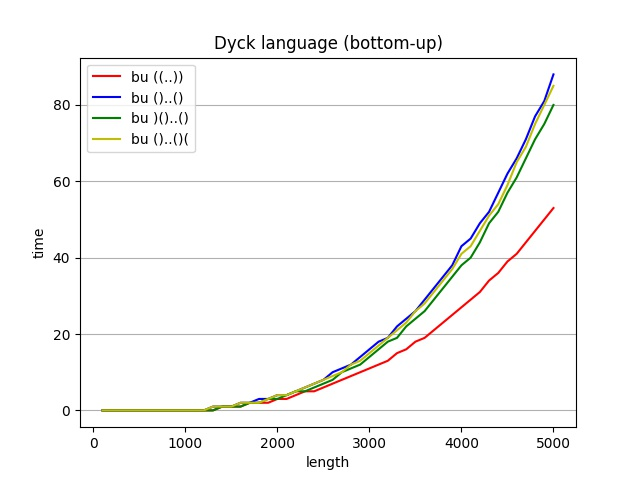
\includegraphics[width=0.6\textwidth]{Resources/t_dyck_bu.jpg}
    \caption{Running time (s) of the bottom-up algorithm when parsing different set of strings of sizes 100-5000, in steps of hundred, for the \textit{Dyck language}.}
    \label{fig:t_dyck_bu}
\end{figure}

Figure~\ref{fig:t_dyck_bu} shows the running times of the bottom-up parser on different sets of input strings.
The strings were of length 100 to 5000, growing in steps of 100.
As we assumed, the times are very similar for all four different sets of input strings.
Parsing the strings of the form \lq((..))\rq~is a little faster.
\todo{This may be, since... maybe this changes with the new brakpoint. analyse new plots. Otherwise consult one note}

The curves are asymptotically to $O(n^3)$, in fact, the yellow, blue and green line are very close to $6.4*10^{-10}*n^3$.

We split the parsings of top-down into two plots.
The first one, Figure~\ref{fig:t_dyck_td_slow}, is for the slow cases, where we did not run the parser on strings longer than 2500
The second one, Figure~\ref{fig:t_dyck_td_fast}, was for the fast cases, where we extended the test set to contain strings up to a size of 10000.

\begin{figure}[h!]
    \centering
    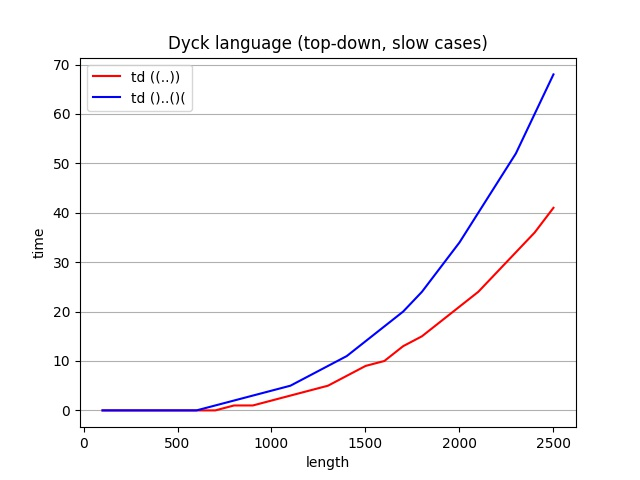
\includegraphics[width=0.6\textwidth]{Resources/t_dyck_td_slow.jpg}
    \caption{Running time (s) of the top-down algorithm when parsing two set of strings of sizes 100-2500, in steps of hundred, for the \textit{Dyck language}.}
    \label{fig:t_dyck_td_slow}
\end{figure}

\begin{figure}[h!]
    \centering
    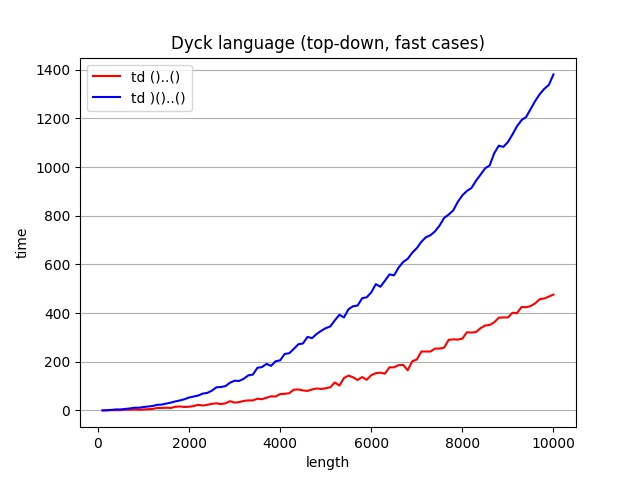
\includegraphics[width=0.6\textwidth]{Resources/t_dyck_td_fast.jpg}
    \caption{Running time (ms) of the top-down algorithm when parsing two set of strings of sizes 100-10000, in steps of hundred, for the \textit{Dyck language}.}
    \label{fig:t_dyck_td_fast}
\end{figure}

As we assumed, parsing the test sets of strings of the form \lq((..))\rq~and \lq()..()(\rq~with top-down was a lot slower than parsing the strings of the other two sets.
While parsing strings of the form \lq()..()(\rq~of length 2500 took almost 70 seconds, parsing strings of the form \lq()..()\rq~of length 10'000 took only 0.4 seconds.

The fast cases are a lot faster than the bottom-up parser.
This is the case, because bottom-up fills all cells of $tab$, regardless of whether or not they are needed to find the solution, while top-down only fills the one needed to find the optimal solution.
When the productions of the grammar are in a favorable order and the splitting points for finding subproblems that yield the optimal solution is low, as it is the case in the fast cases of Dyck, it can be very fast.

However, if this is not the case, then the parser may take a lot of time.
We can see this at the slow cases of the \textit{Dyck language}.
Here, the parser behaves a lot worse than bottom-up.
This may be due to the fact, that bottom-up fills the cells of $tab$ in a structured way, accessing the already filled cells of $tab$ not more often, then needed to fill the other cells.
Top-down on the other hand may run into the same subproblems very often.
This means the algorithm calls itself recursively in order to access the cell of the same subproblem more often than bottom-up does.
Since recursive calls are more time consuming, and more accesses may be performed, this results in a potentially very bad running time.

\begin{figure}[h!]
    \centering
    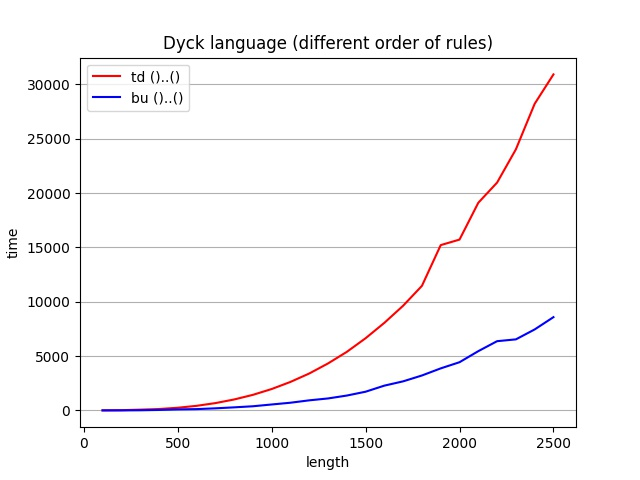
\includegraphics[width=0.6\textwidth]{Resources/t_dyck_order.jpg}
    \caption{Running time (ms) of both algorithms for parsing a set of strings of sizes 100-2500, in steps of hundred, for the \textit{Dyck language}, with a different order of the productions.}
    \label{fig:t_dyck_order}
\end{figure}

I order to verify the hypothesis, that the order of productions matters for the top-down parser, we run experiments on the same grammar, but with the productions of $S$ in opposite order.
The results can be seen in figure~\ref{fig:t_dyck_order}.
The parser is in fact a lot slower than it was before, thus the order of the productions may play a major role, when parsing.
The plot further shows that the order does not matter that much for the bottom-up parser.
It has almost the same running time, than it had with the original ordering of the productions.

\subsection{Strings starting and ending in a}

The running times achieved, did not meat all expectations.
Surprisingly, both the top-down and bottom-up algorithm performed very differently on the two grammars, being very fast at parsing for the grammar \textit{starting in a}, and slower for \textit{ending in a}.
In general, we see that the times are lower than they were for the \textit{Dyck language}.
This is presumably because this grammar has only two non-terminal productions, which leads to less subproblems which have to be considered.

We split the results in three graphs; one for the running times of both parsers on the grammar \textit{ending in a} (Figure~\ref{fig:t_ea_td_bu}), one for top-down and one for bottom-up, each for the grammar starting in a (Figure~\ref{fig:t_sa_td} and ~\ref{fig:t_sa_bu} respectively).

\begin{figure}[h!]
    \centering
    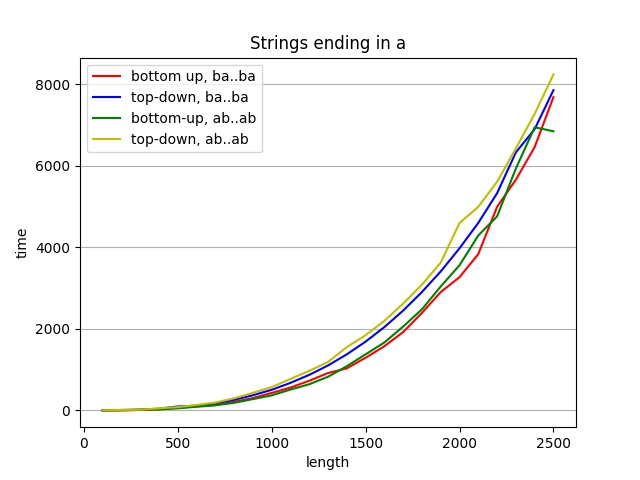
\includegraphics[width=0.6\textwidth]{Resources/t_ea_td_bu.jpg}
    \caption{Running time (ms) of the bottom-up and top-down algorithm when parsing two set of strings of sizes 100-2500, in steps of hundred, for the Language of words ending in a.}
    \label{fig:t_ea_td_bu}
\end{figure}

We see, that the curves for parsing the grammar \textit{ending in a} are almost identical with the ones of the bottom-up parser run on the \textit{Dyck language}.

\begin{figure}[h!]
    \centering
    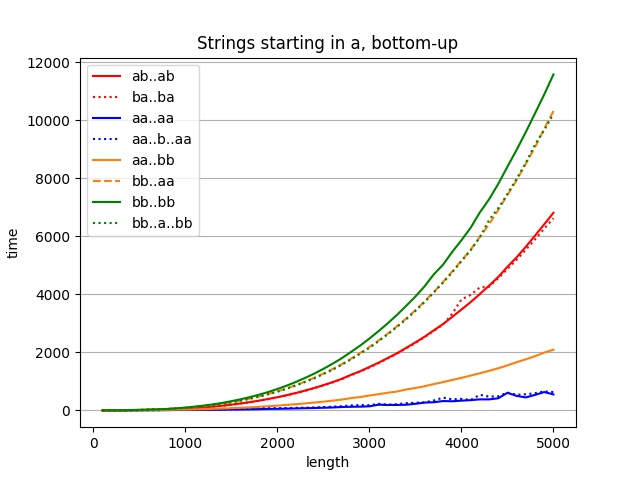
\includegraphics[width=0.6\textwidth]{Resources/t_sa_bu.jpg}
    \caption{Running time (ms) of the bottom-up algorithm when parsing two set of strings of sizes 100-2500, in steps of hundred, for the Language of words starting in a.}
    \label{fig:t_sa_bu}
\end{figure}

However, the running times for the grammar \textit{starting in a} are a lot faster.
If we consider how $tab$ will be filled by the algorithm, it becomes clear, why that is.
Remember that $tab$ for this grammar is $3\times n\times n$, since it has three non-terminal variables.
We look at the two dimensional table of each non-terminal in turn.

The table for $A$, say $tab_A$, has \textit{true} only in the row for substrings of length 1 and where the symbol is \lq a\rq.
As it has no non-terminal production, when trying to fill the reminder of $tab_A$ the algorithm proceeds very fast, since no splitting has to be considered, as the corresponding loop over $k$ is never even accessed.

The table for $B$, $tab_B$, has \textit{true} in all cells.
All substrings of length one can be yielded, since $B$ has the two terminal productions $B\rightarrow a|b$.
Further, since its only non-terminal production is $B\rightarrow BB$, when trying to fill a new cell of $tab_B$, only other cells of $tab_B$ must be considered.
Because they are all \textit{true}, the loop over the splitting point $k$ gets braked after the first splitting point, thus filling $tab_B$ can be done in a slow matter, too.

Let's now look at $tab_S$.
Since the only production for $S$ is $S\rightarrow AB$, first the cell of $tab_A$ gets accessed.
The first splitting point always generates a substring of length one, on the left of $k$.
If this is an \lq a\rq, then the corresponding cell in $tab_A$ is \textit{true}, and we must access $tab_B$ as well.
As we argued before, this value will always be \textit{true}, we are thus not looking at any other splitting points.
If the substring is b, then the cell in $tab_A$ is \textit{false}, and we will not look at $tab_B$, but continue to the next splitting point.

For the grammar \textit{ending in a}, $tab_A$ and $tab_B$ are filled in a very similar manner.
However, when filling $tab_S$ we have almost twice the amount of table accesses to $tab_B$.
Since the production for $S$ is $S\rightarrow BA$, for every splitting point first $tab_B$ gets accessed, which will always return \textit{true}, and then $tab_A$ gets accessed, which will return \textit{false} in most cases.
Thus, both $tab_B$ and $tab_A$ are accessed for every $k$, while for \textit{starting in a} $tab_B$ was only accessed when $tab_A$ was \textit{true}.

For \textit{starting in a}, we expect very similar running times for strings of the form \lq aa..bb\rq~and \lq bb..aa\rq.
For \textit{ending in a}, we expect worse running times for those strings.
We expect it to be even worse for strings of the form ab..bb, while for strings starting in a it would result in a similar running time.
\todo{run experiments, include plots}


\begin{figure}[h!]
    \centering
    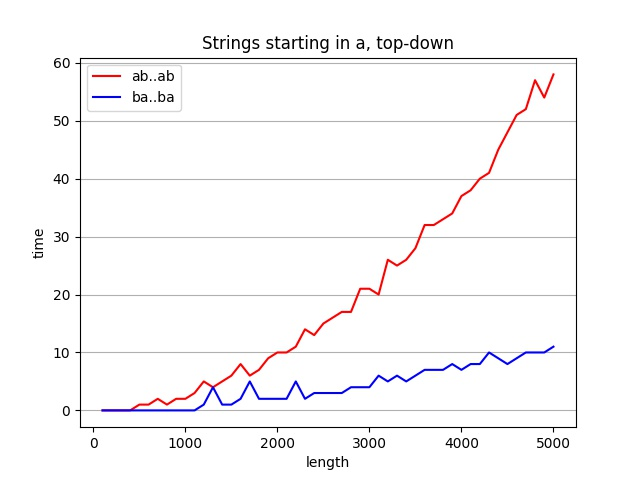
\includegraphics[width=0.6\textwidth]{Resources/t_sa_td.jpg}
    \caption{Running time (ms) of the top-down algorithm when parsing two set of strings of sizes 100-5000, in steps of hundred, for the Language of words starting in a.}
    \label{fig:t_sa_td}
\end{figure}

As we see in Figure~\ref{fig:t_sa_td}, the running times for top-down were incredibly low.
The three bumps in the blue line are supposedly due to rounding errors of the compiler, seen as the times there are lower than 5 milliseconds.
The bumps appear on the red line at the same time after the same period of time after starting the parsers (not at the same length!), though not as distinctive as in the blue line, since the running times are already a little higher at this point.
They could also be reduced by running the parser 40 times per input string instead of the 10 times used in all other experiments.

The incredibly low running times can be explained with similar reasoning, as for the low running times of bottom-up on strings starting with a.
Top-down is even faster, since it does not fill $tab$ completely.
In fact, when parsing strings not starting in \lq a\rq~for the grammar \textit{starting in a}, it will only ever look at the most left children of the recursive tree, since each of them returns \textit{false}
This results in a very low amount of recursive calls.
In fact, the number of calls on the recursive function is $\Theta(n)$ (figure~\ref{fig:c_sa_td}).
As we argued in section~\ref{sec:top_down}, the upper bound for this number is $O(n^3)$.
The numbers for the counter of bottom-up (repetitions of the inner most loop, i.e. over splitting points $k$) for parsing strings for the grammar starting in a, are somewhere in the middle of $n^2$ and $n^3$, still yielding relatively fast running times.
\todo{adapt, if new break in bottom up is used.}

\begin{figure}[h!]
    \centering
    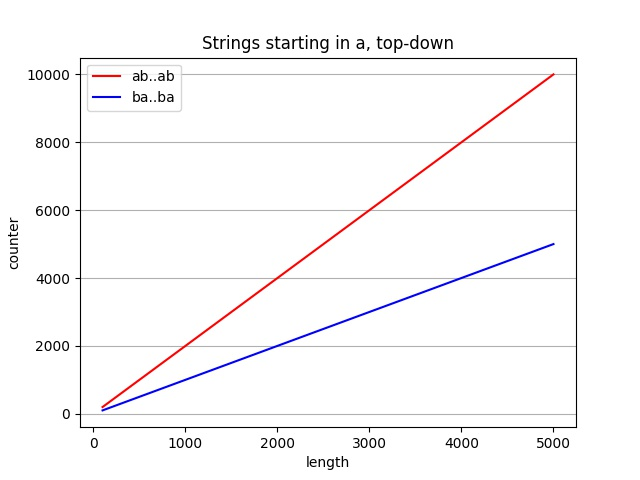
\includegraphics[width=0.6\textwidth]{Resources/c_sa_td.jpg}
    \caption{Running time (ms) of the top-down algorithm when parsing two set of strings of sizes 100-5000, in steps of hundred, for the Language of words starting in a.}
    \label{fig:c_sa_td}
\end{figure}
\todo{add evaluation for \textit{equal numbers}}
\todo{Add subsection for evaluations of step 3}



